\section{Tests of additional meta-parameters}
\lb{sec:app}

In this appendix we discuss tests of some meta-parameters, which had a relatively little effect on the 
accuracy of the algorithms. For these tests we use the 2-class classification in the 3FGL catalog.

For the LR algorithm, we test two additional meta-parameters: regularization and tolerance. 
The effect of the choice of these parameters on accuracy is less than 1\% (Fig. \ref{fig:LR_tol_reg}). 
Therefore we used the default values for these parameters (tolerance is $10^{-4}$ and regularization parameter is 1)
both in the 2-class and in the 3-class classifications.

\begin{figure}[h]
\centering
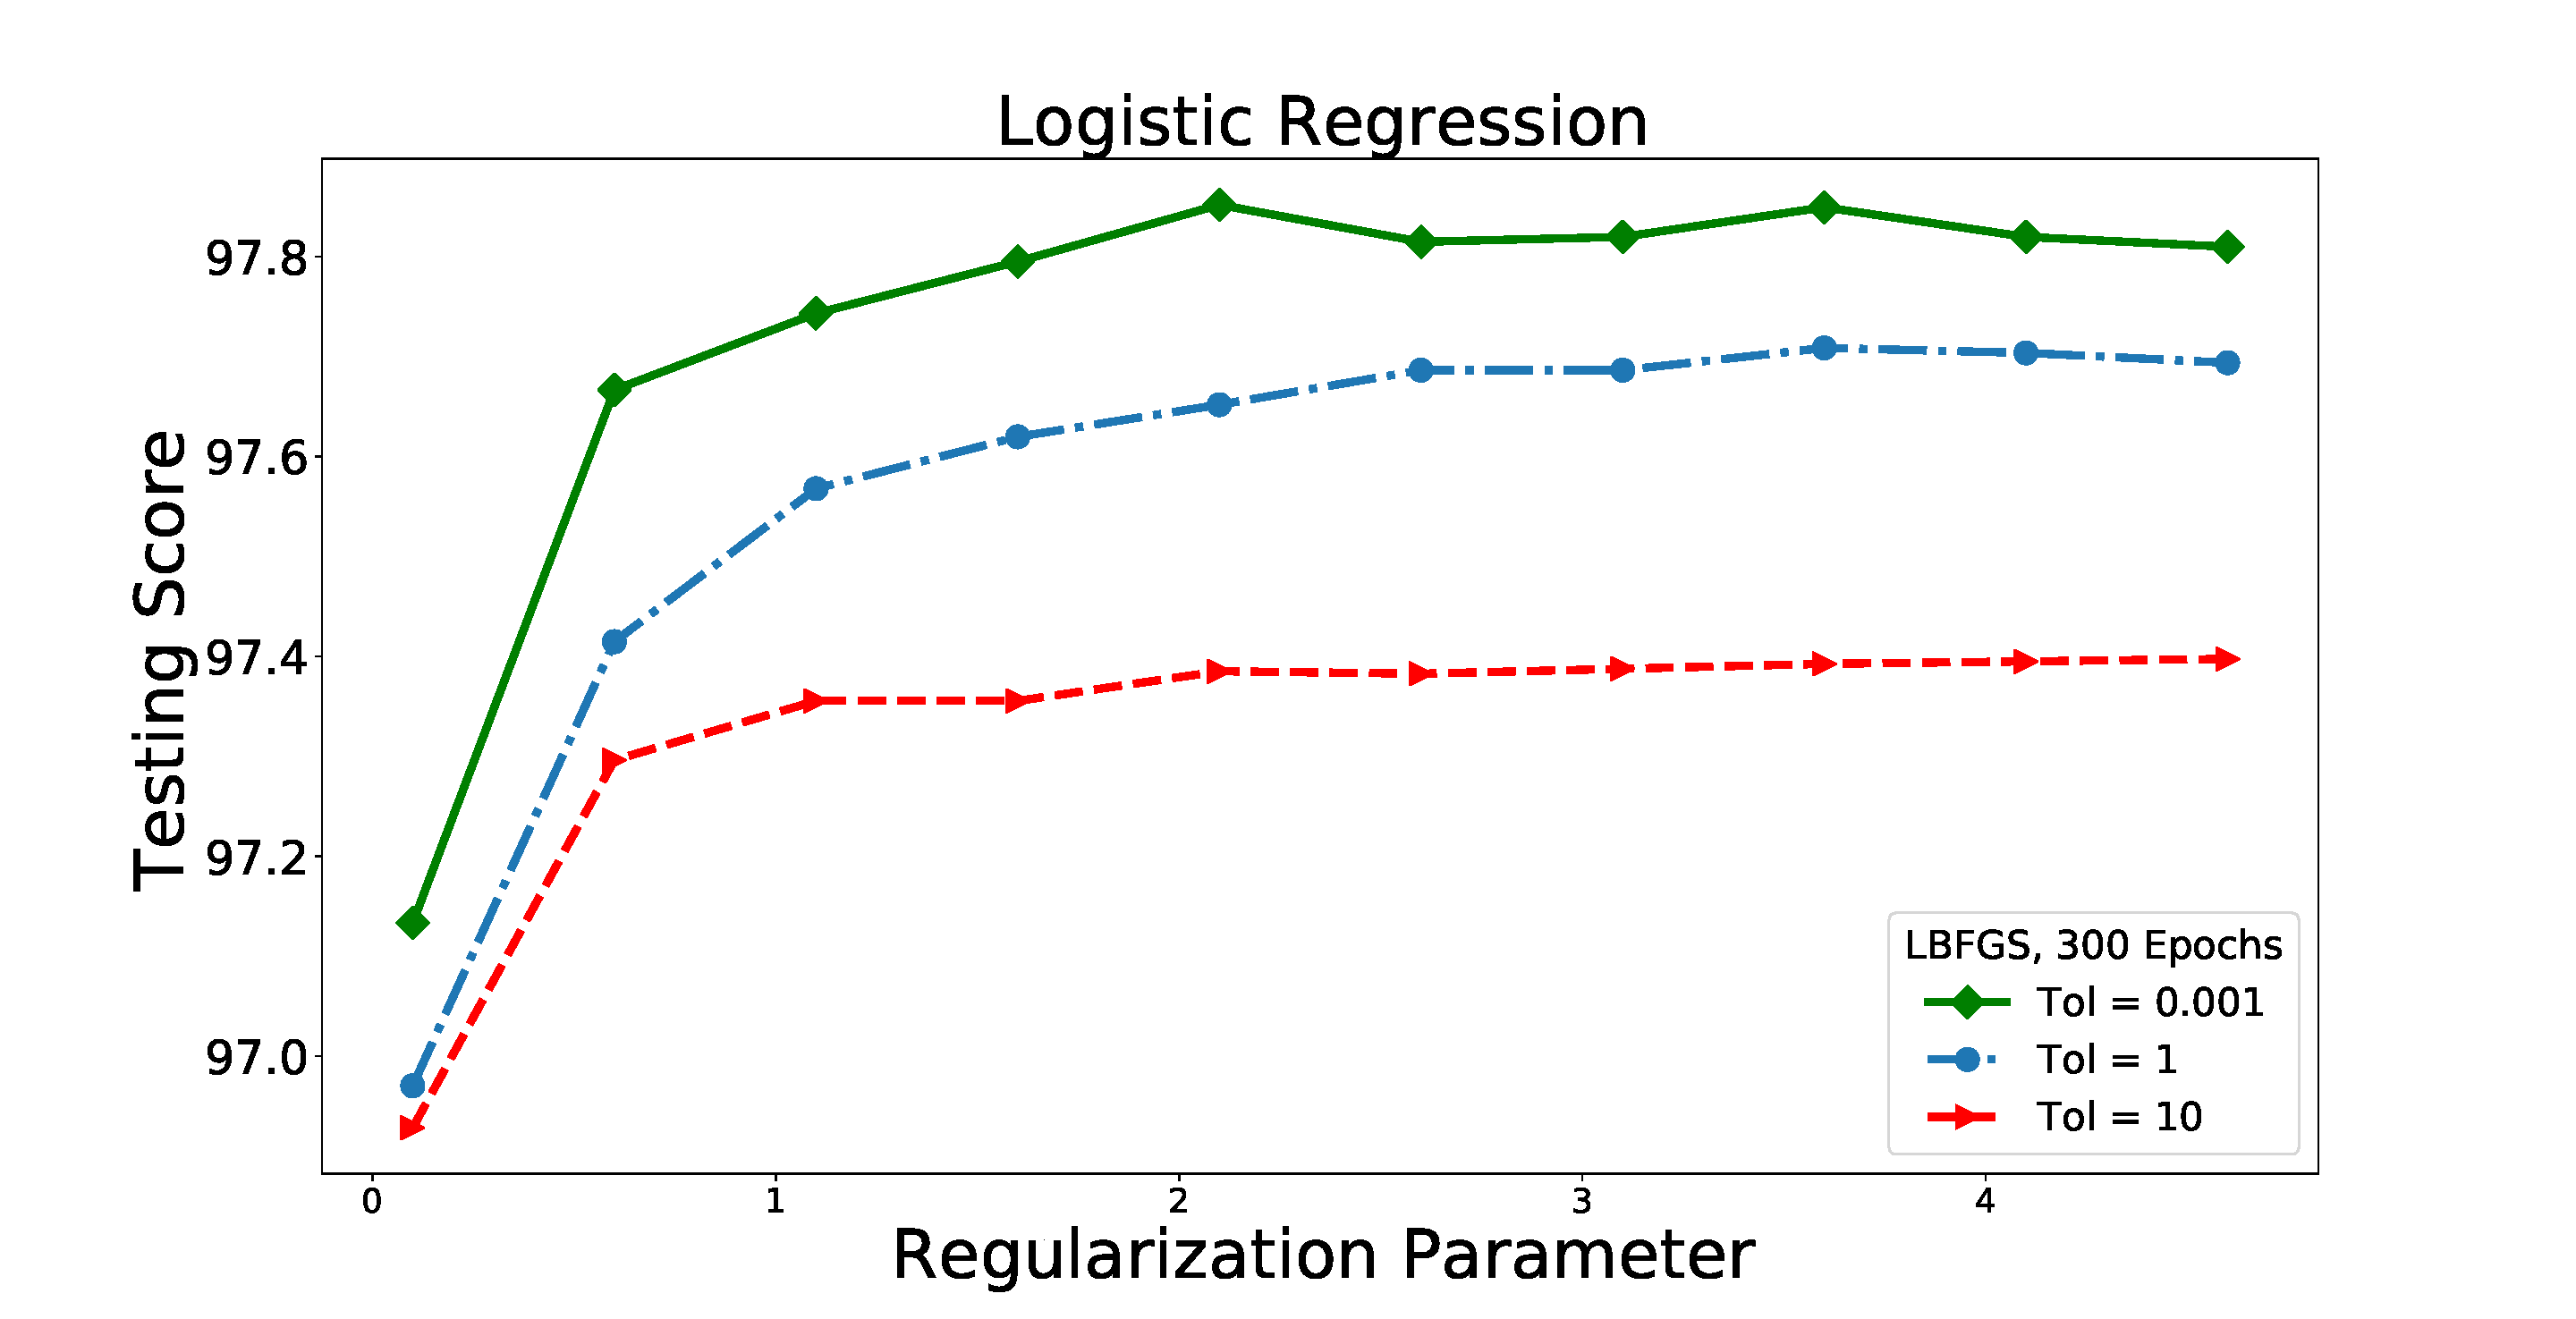
\includegraphics[width=\twopicsp\textwidth]{plots/lr_train_reg.pdf}
\caption{Dependence of LR on tolerance and regularization. 
}
\label{fig:LR_tol_reg}
\end{figure}

In Fig. \ref{fig:nn_nn} we show the effect of adding the second hidden layer in the NN algorithm.
The difference between the best accuracies of the NN with one hidden layer (cf. Table \ref{tab:selected_algs})
and  the NN with the additional hidden layer is less then 1\%.
\begin{figure}[h]
\centering
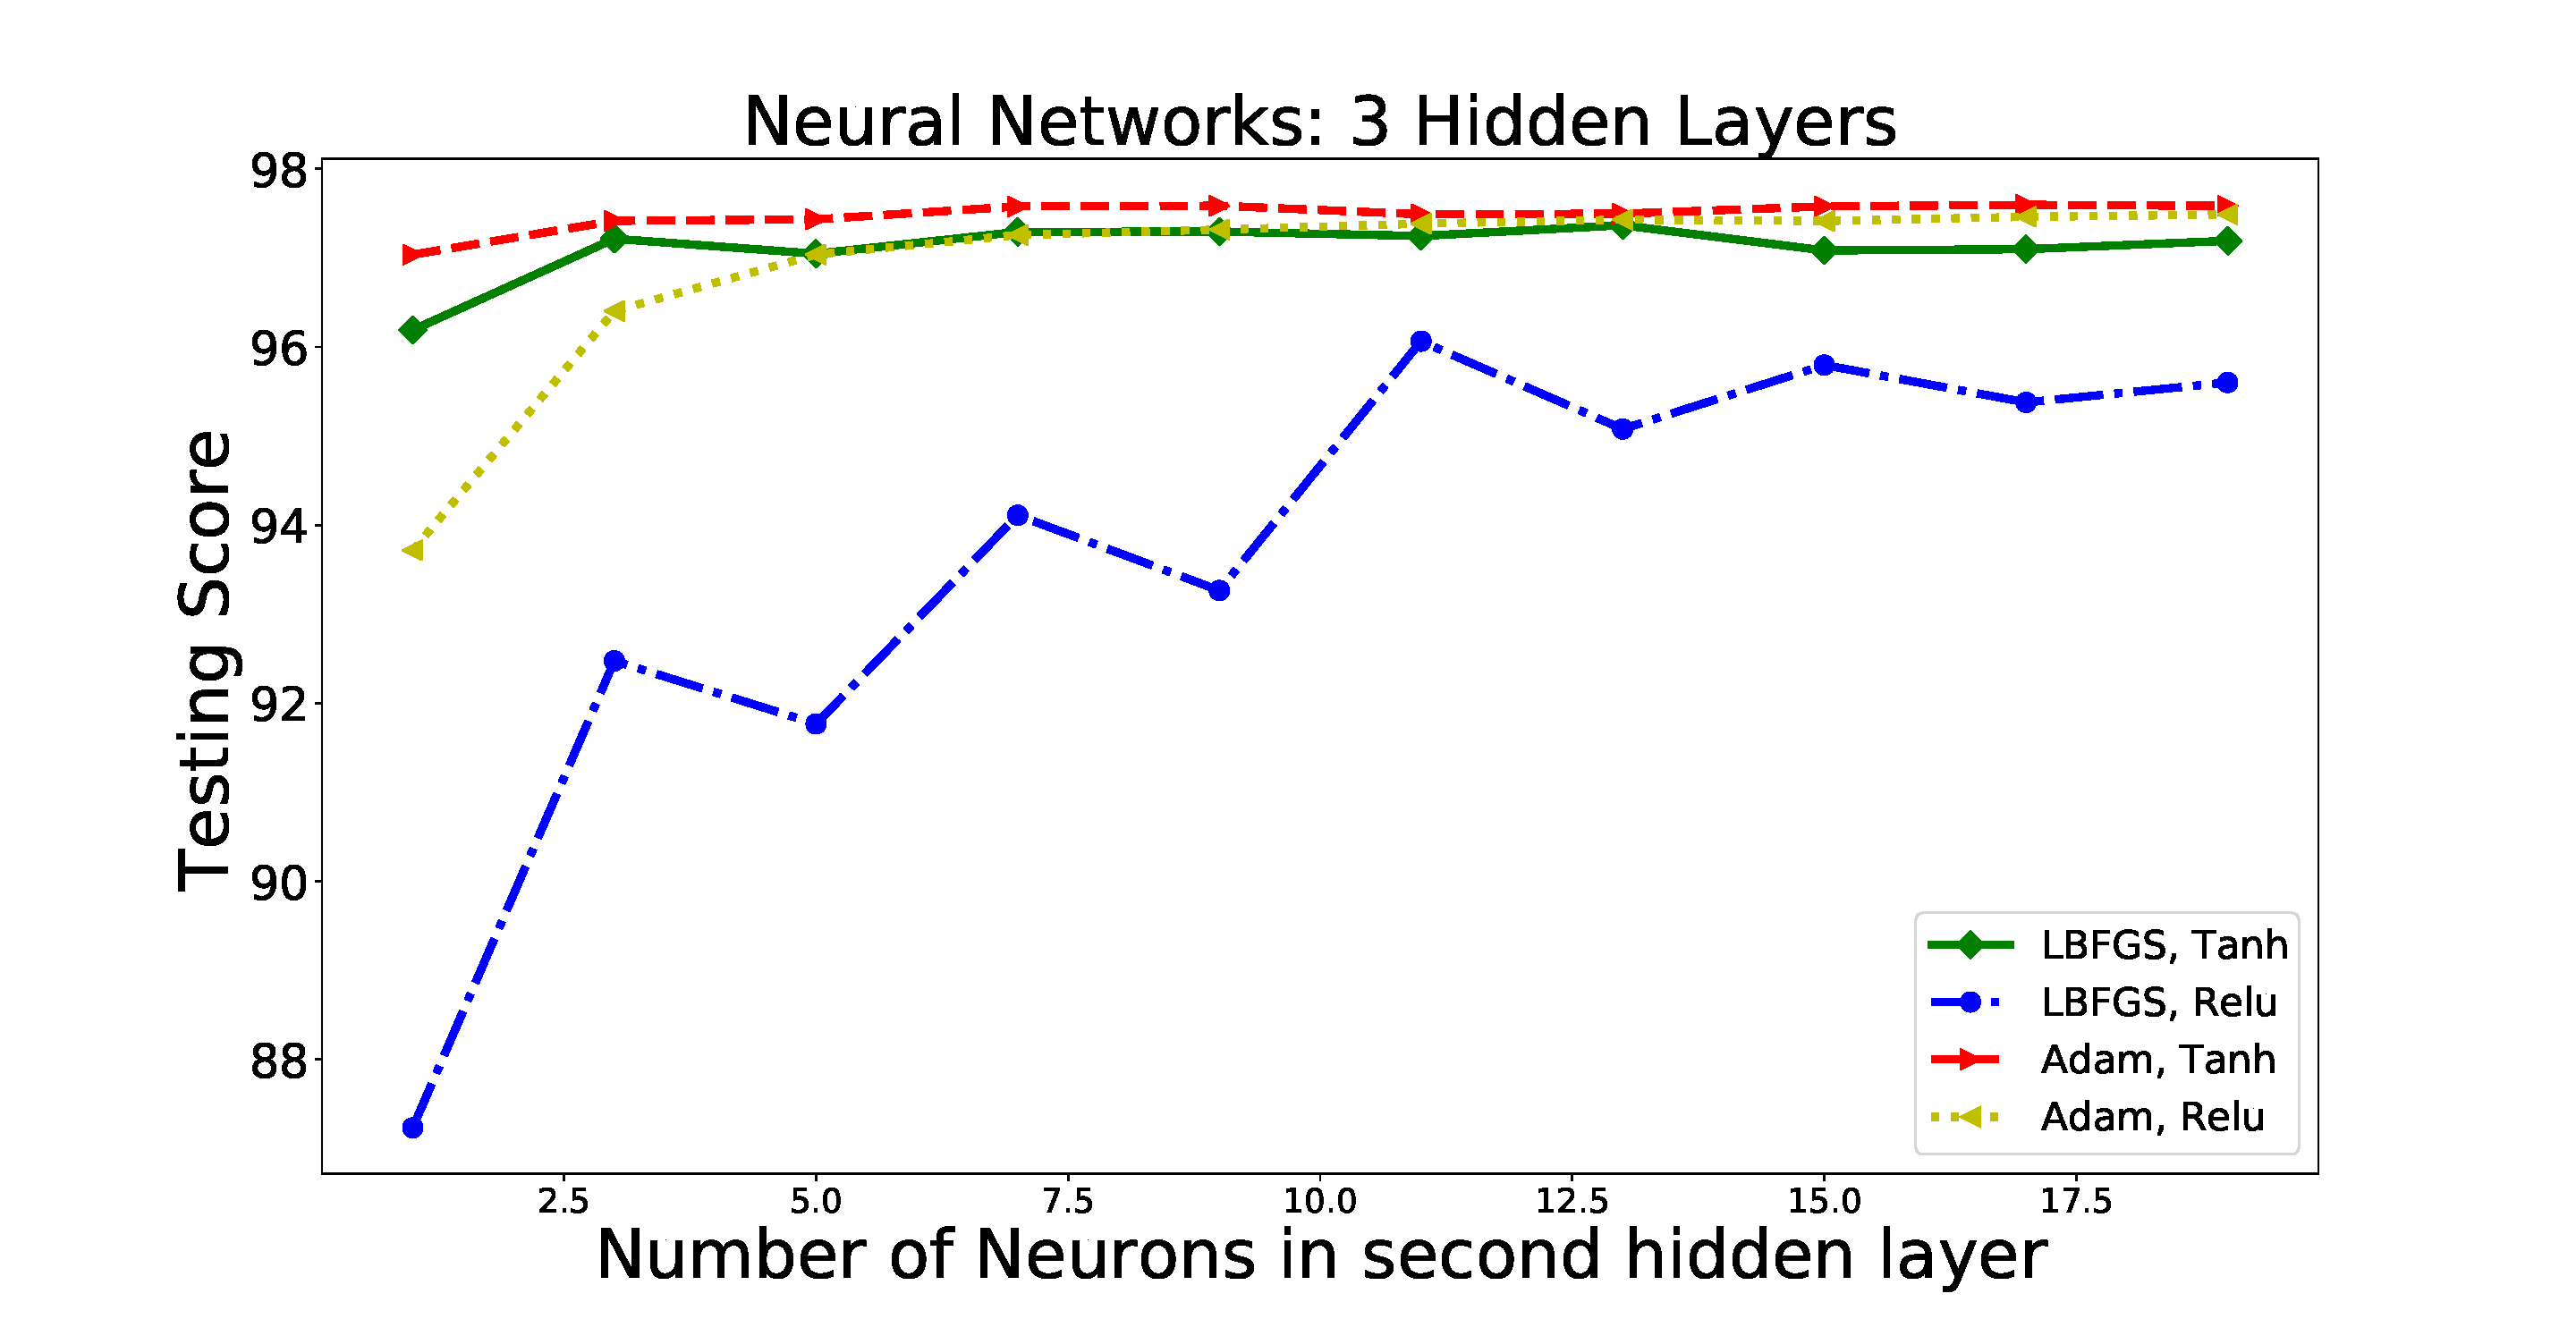
\includegraphics[width=\twopicsp\textwidth]{plots/nn_2layers_3fgl.pdf}
\caption{Dependence of NN on the number of neurons in the second hidden layer, for 11 neurons in the first hidden layer.
}
\label{fig:nn_nn}
\end{figure}


\pgfplotstableread[col sep=comma]{tables/features/3fglassocfeaturesAGNPSRnewfeats.csv}\tablea
\begin{table}
\centering
\resizebox{0.45\textwidth}{!}{
\pgfplotstabletypeset[
columns={Name,Mean,SD,Minimum,Maximum},
column type=c,
string type,
every head row/.style={before row=\hline\hline,after row=\hline,},
every last row/.append style={after row={\hline} },
every first column/.style={column type/.add={}{}},
every last column/.style={column type/.add={}{}},
columns/Name/.style={column name=Feature Name,string replace*={_}{\textunderscore}},
columns/Mean/.style={column name=Mean,column type=c,numeric type,fixed,precision=2},
columns/SD/.style={column name=Standard Deviation,numeric type,fixed,precision=2},
columns/Minimum/.style={column name=Minimum,numeric type,fixed,precision=2},
columns/Maximum/.style={column name=Maximum,numeric type,fixed,precision=2},
skip rows between index={11}{25}
]{\tablea}
}
\vspace{2mm}
\caption{Statistics of features used for 2 class probabilistic classification of the 3FGL sources.
\lb{tab:3FGL_features}}
\end{table}

\pgfplotstableread[col sep=comma]{tables/features/4fgldr2agnpsrfeatures.csv}\tableaf
\begin{table}
\centering
\resizebox{0.45\textwidth}{!}{
\pgfplotstabletypeset[
columns={Name,Mean,SD,Minimum,Maximum},
column type=c,
string type,
every head row/.style={before row=\hline\hline,after row=\hline,},
every last row/.append style={after row={\hline} },
every first column/.style={column type/.add={}{}},
every last column/.style={column type/.add={}{}},
columns/Name/.style={column name=Feature Name,string replace*={_}{\textunderscore}},
columns/Mean/.style={column name=Mean,column type=c,numeric type,fixed,precision=2},
columns/SD/.style={column name=Standard Deviation,numeric type,fixed,precision=2},
columns/Minimum/.style={column name=Minimum,numeric type,fixed,precision=2},
columns/Maximum/.style={column name=Maximum,numeric type,fixed,precision=2},
]{\tableaf}
}
\vspace{2mm}
\caption{Statistics of features used for 2 class probabilistic classification of the 4FGL-DR2 sources.
\lb{tab:4FGL_features}}
\end{table}


\begin{table}[!h]
\tiny
\centering
\renewcommand{\tabcolsep}{1mm}
\renewcommand{\arraystretch}{1}

\begin{tabular}{c c c}
\hline
\hline
Feature & RF: 50, 6& BDT: 100, 2\\
\hline
{ $\ln$(LP\_SigCurv)}&  0.297  & 0.465   \\
{LP\_beta}&0.151&0.109\\
{ $\ln$(Variability\_Index)} &0.085& 0.253   \\
$\ln$(Unc\_Energy\_Flux100)& 0.081&0.059  \\
$\ln$(Energy\_Flux100) & 0.076&0.008   \\
HR56&0.071& 0.015  \\
Unc\_LP\_Index & 0.067&0.009  \\
HR34& 0.035&0.005  \\
$\ln$(Pivot\_Energy)&0.031&0.006\\
HR23 &0.025& 0.005     \\
 LP\_Index& 0.015&0.016  \\
HR67&0.015&0.010\\
HR45&0.015&0.006\\
GLON&0.013&0.017\\
HR12&0.009&0.004\\
GLAT&0.007&0.003\\
\hline
\end{tabular}
\vspace{2mm}
\caption{Feature importances for classification of 4FGL-DR2 sources using
RF (50 trees, max depth 6) and BDT (100 trees, max depth 2) algorithms
ordered by decreasing importance 
in the case of RF algorithm.
}
\label{tab:feat_imp2}
\end{table}



We summarize features and their statistics,
which we use for probabilistic classification of sources in the 3FGL and 4FGL-DR2 catalogs
in Tables \ref{tab:3FGL_features} and \ref{tab:4FGL_features} respectively. 
We show the feature importances for the 2-class classification of 4FGL-DR2 sources in Table \ref{tab:feat_imp2}.
Similarly to feature importances for the 3FGL 2-class classification reported in Table \ref{tab:feat_imp}, 
some of the most important features are significance of curvature in the spectrum, variability index, energy flux above 100 MeV and its uncertainty.

\section{Comparison of Oversampling methods}

Here we compare the oversampling method we use in our catalog with the SMOTE oversampling technique. SMOTE oversamples by creating synthetic data based on the data points already available. For a direct comparison we used the associated sources in 4FGL-DR2 and compared the probabilities of the individual sources. We calculate normalized differences of individiual probabilities $P_{D}$ by the formula:

\begin{align}
P_{D}= \frac{\Delta}{max(\sigma_{O},\sigma_{S})}
\end{align}

where $\Delta$ is the difference of probabilities for the normal oversampling (O) and the SMOTE oversampling (S), for individual methods. We then plot a histogram for this value. One would expect a difference of 0.0 and a standard deviation of 0.5 for there to be no statistical difference between the two methods. The table below shows the parameters:
\begin{table}[!h]
\tiny
\centering
\renewcommand{\tabcolsep}{1mm}
\renewcommand{\arraystretch}{1}

\begin{tabular}{c c c}
\hline
\hline
Method & Mean&Std.\\
\hline
RF& -0.250 & 0.451\\
\hline
BDT&-0.040&0.511 \\
\hline
NN&0.555&0.573\\
\hline
LR&0.617&0.644\\
\end{tabular}
\vspace{2mm}
\caption{The Parameters of histograms for the 4 algorithms used.
}
\label{tab:compO}
\end{table}

We plot here the histogram for BDT and LR:
\begin{figure}[h]
\centering
\hspace*{-1cm}
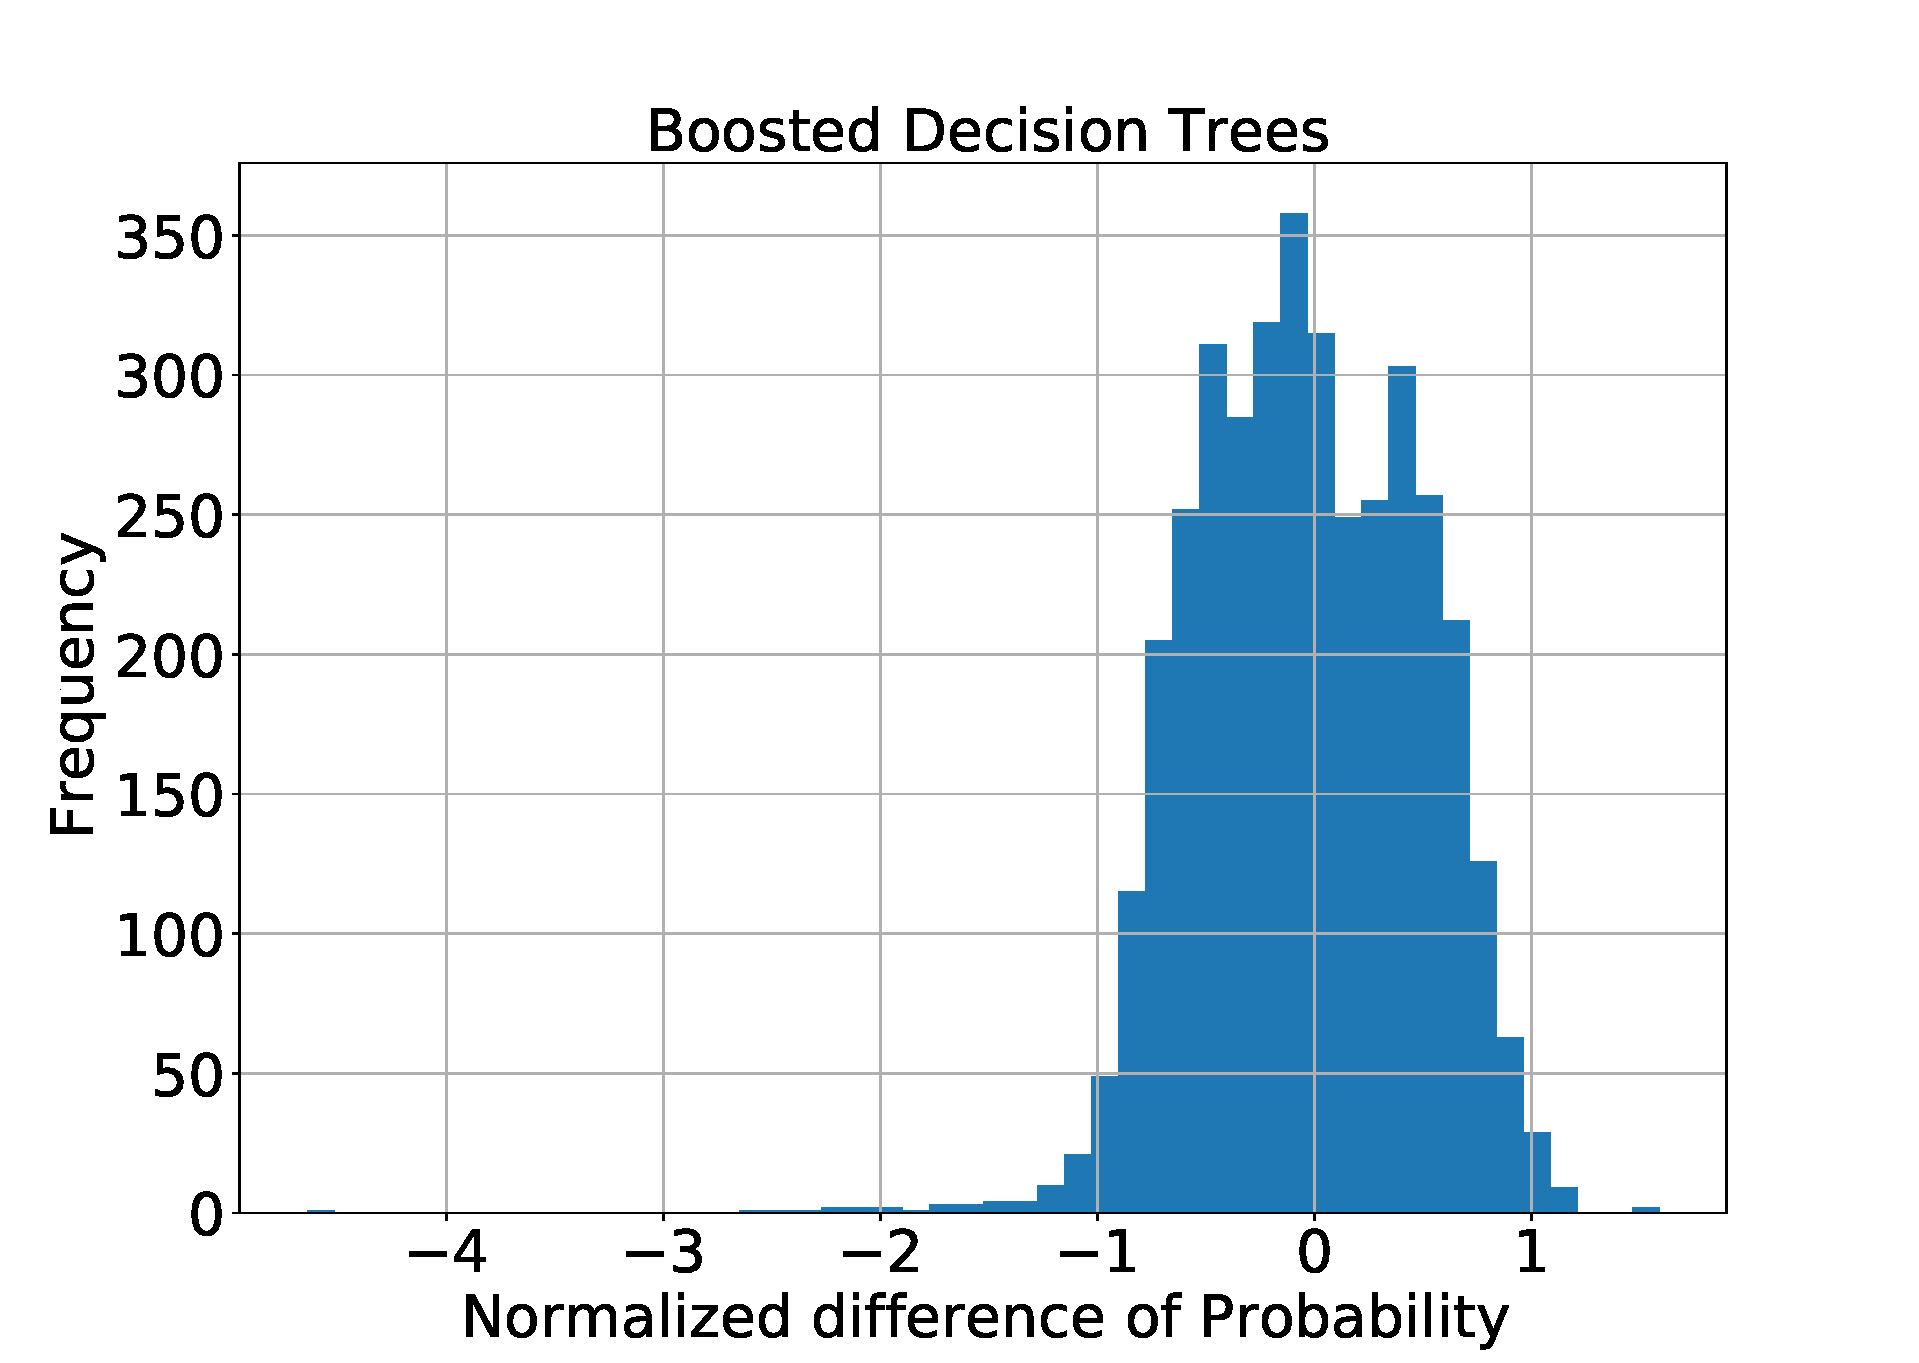
\includegraphics[width=0.55\textwidth]{plots/diffBDT2.pdf}
\caption{Histogram for comparison of oversampling with BDT.
}
\label{fig:nn_nn}
\end{figure}

